\section{Motionplanning}
%When stockfish has provided a move for the robot,


\subsection{ROS2 and Moveit2}
ROS2 (Robot Operating System 2) is a middleware solution meant for working with robots.\cite{ROS} It can handle multiple programs, called nodes, at once that communicate using publishers and subscribers on topics to effectively parallelize processes. To handle communication with the robot, the Universal Robots UR ROS2 driver is used. This driver communicates with the robot using the RTDE protocol and an external control URcap,\cite{URDriver} with which it updates the robot state with a frequency of 125 Hz, as well as sending trajectories for the robot. The UR driver provides an interface for the robot which Moveit2 can access to provide motionplanning.

\begin{figure} [H]
    \centering
    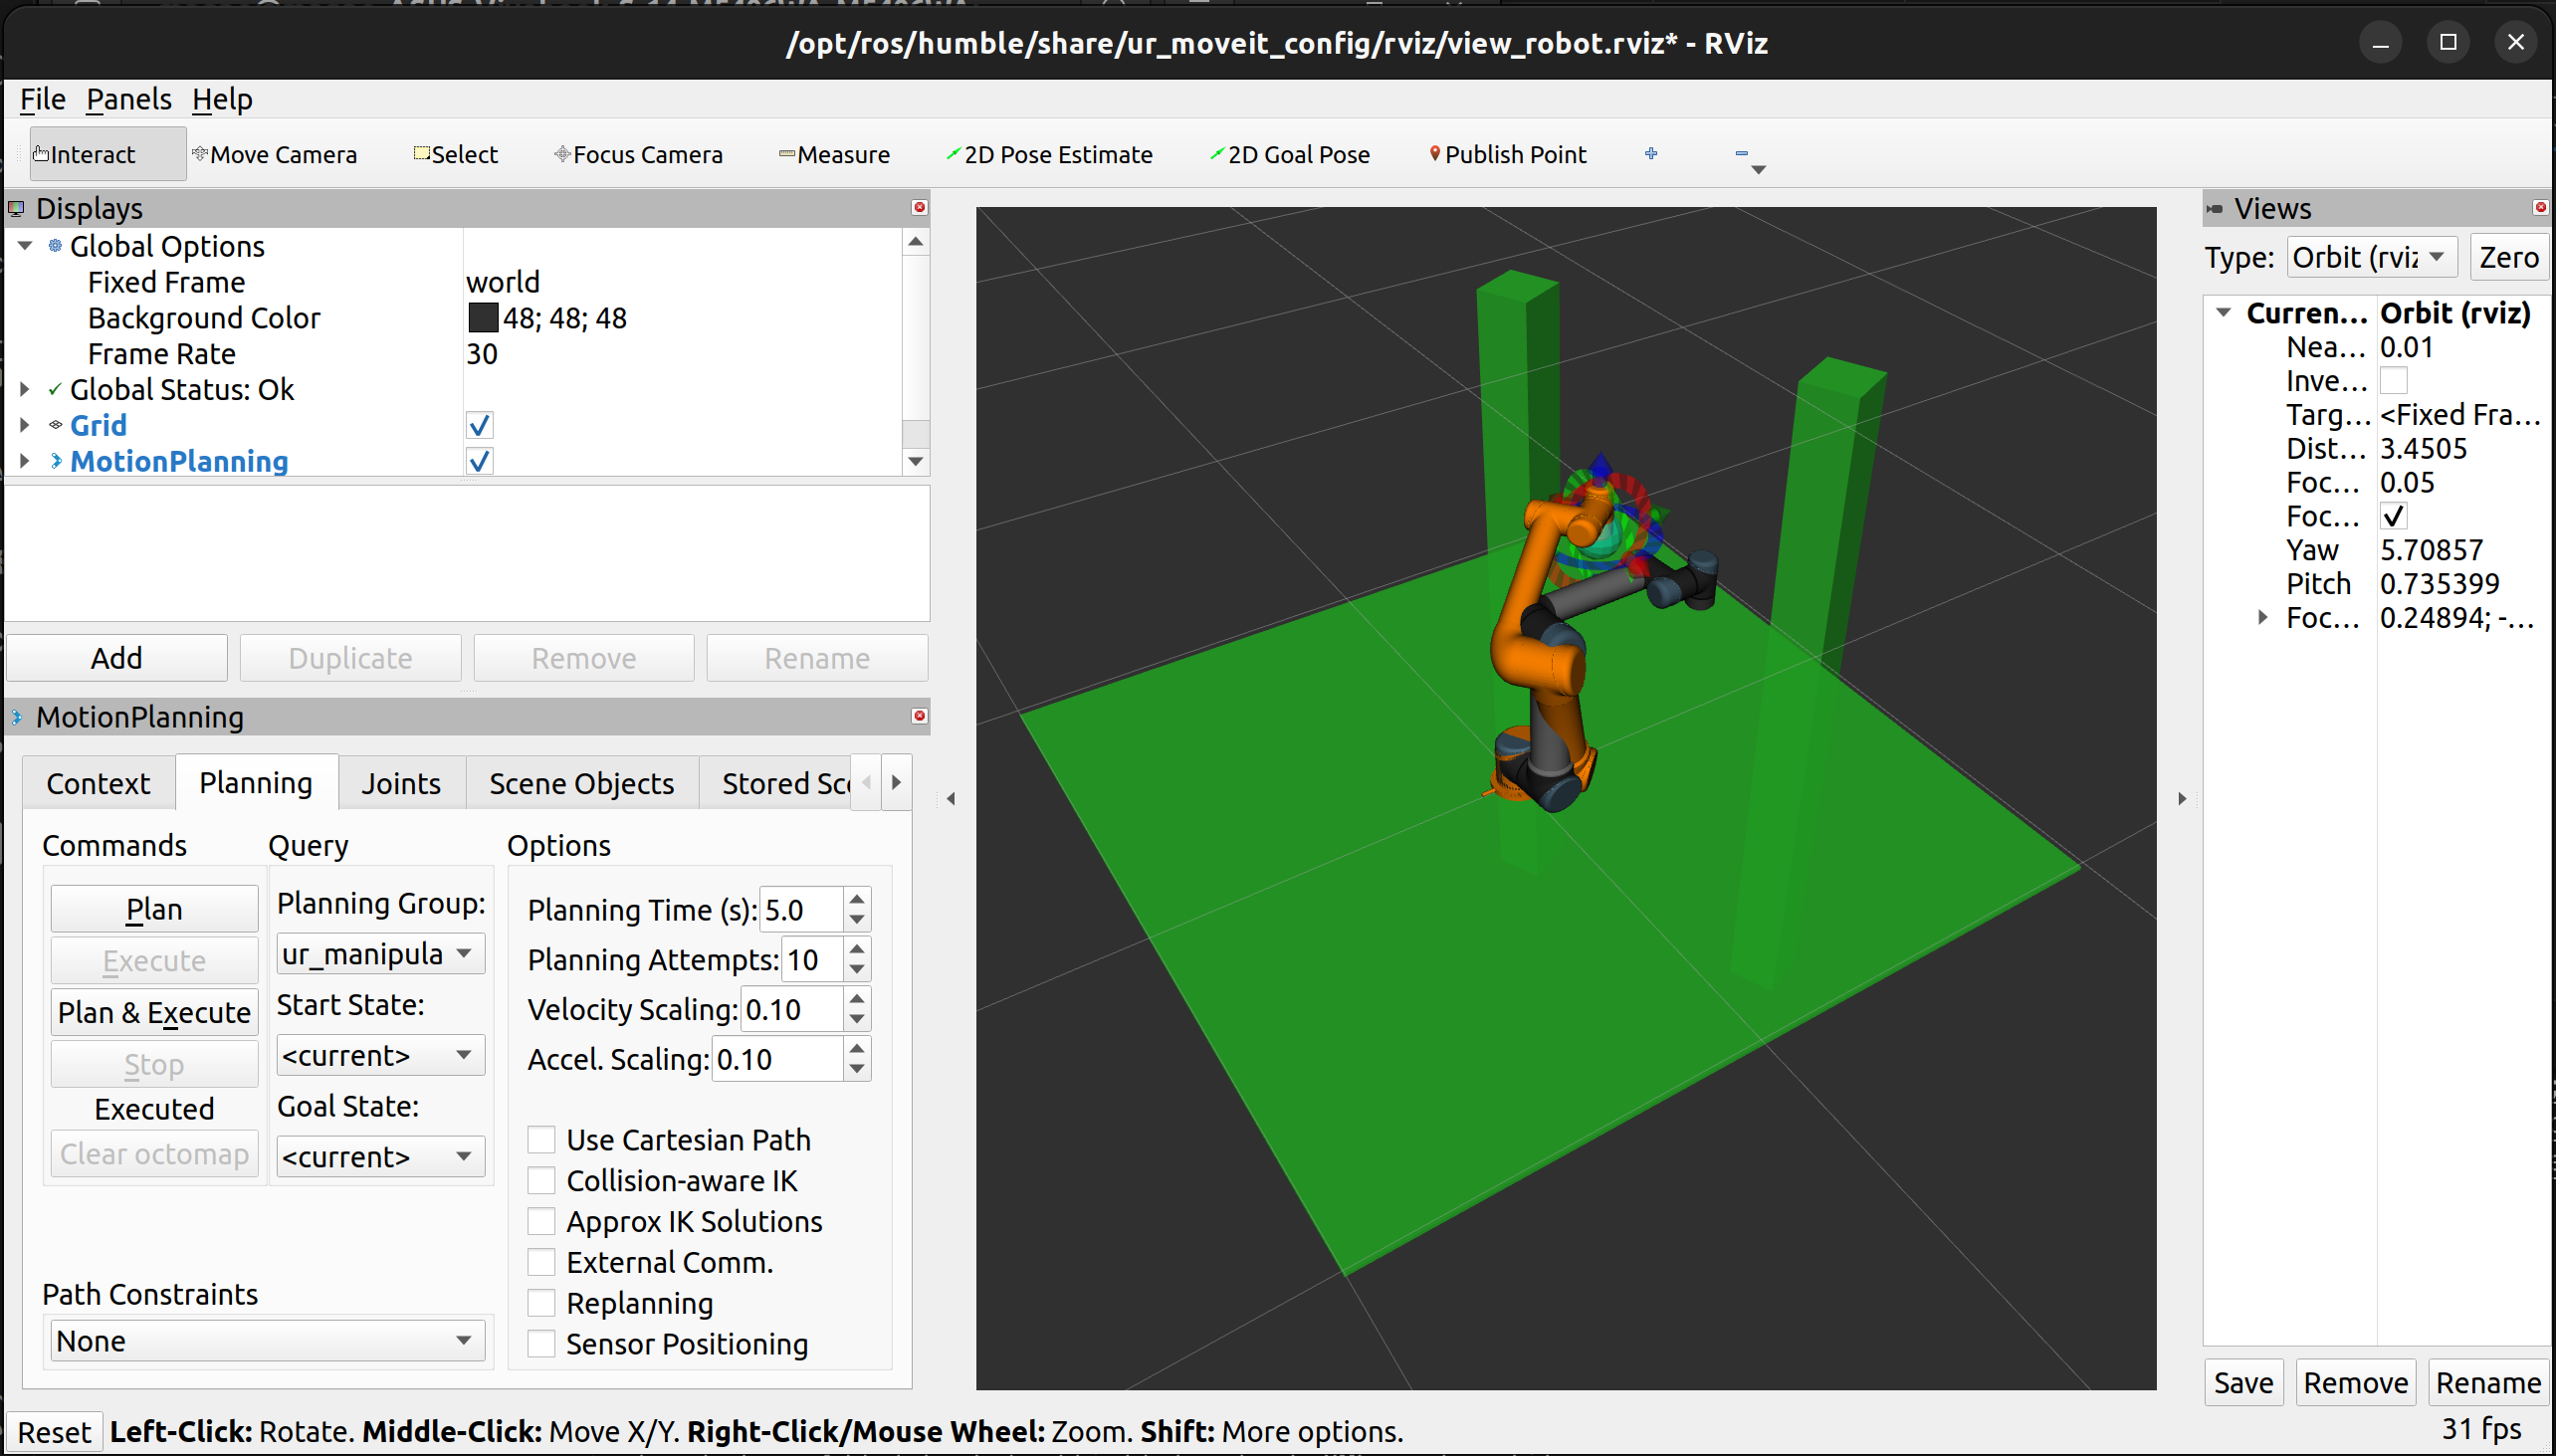
\includegraphics[width=0.7\linewidth]{Pictures/Rviz-screenshot.png}
    \caption{The visual GUI tool Rviz for ROS2, set up with obstacles and Moveit2}
    \label{fig:Rviz}
\end{figure}

Moveit2 (or Moveit for ROS2) is an interface for ROS2 that handles motionplanning, inverse kinematics and obstacle avoidance for robots.\cite{MoveIt} In addition to providing the driver with a motion planning interface, Moveit2 also provides an extension to the ROS visual GUI tool Rviz, seen in \cref{fig:Rviz}. With this, it is possible to simulate the robot to prototype and plan in a controlled environment.

When moving, the robot's end effector, where the gripper is mounted, will follow a path of waypoints linearly in cartesian space to ensure smooth movement above the other pieces. Using Moveit2, this is done by using a vector of Cartesian poses (including both position and angle of the end affector) and the computeCartesianPath function, where it will discretize the path and update a trajectory for the robot. If the trajectory can be computed, it will execute it using the UR drivers interface, moving the end effector of the robot.

\subsection{Moving pieces}
Any move the robot needs to make can be split into individual moves the robot can handle while only holding one piece at a time. The four essential moves needed are: 

1. Moving a piece from one square to another empty square. 

2. Moving a piece from a square to a death position and adding it to an array. 

3. Finding a dead piece in memory and moving it to an empty square on the board. 

4. Moving a piece the player has captured from a predefined position to a death position and adding it to an array.

All possible moves in chess can be split into these and, as such, those are the four moves that need to be implemented.

In \cref{sec: Workbench setup} the death position-plates can be seen on \cref{fig: workbench setup}. These positions are hardcoded as their place won't change dynamically between games. 
When a piece gets captured, it will be put into one of these positions, whereafter the piece type that was stored there is remembered in case it will be used later for the promotion of a pawn. When a piece is added, it will then search the positions for the piece that will be added and pick up that piece. If multiple pieces of the same type (eg two knights) have been removed from the board the first one captured will be taken.

As the chessboard does not change height throughout the game, only 2 dimensional coordinates are needed for most of the calculations. The z-axis or height of the end effector is only important when picking up pieces and placing them. The heights at which pieces will be picked up on the board and the table are also known before playing and will be static just as the death positions. 

The resulting movement will then be in 3 parts. The first is from a preset idle position to the first point where a piece is picked up. The next is movement holding the piece whereafter the piece is let go. The last is the following move back to the idle position. These follow the linear paths in cartesian space above the board at a travel height, while only moving down to the aforementioned board and table height when picking up and placing pieces.

\subsection{Moving in multiple reference frames}

Using Moveit2 a static transformer can be set up. Static transformers are simple nodes that, at a specified frequency, publish a transformation matrix to a reference frame to be used for cartesian poses.\cite{6556373} The static transformer set up for the project provides a frame rotated $112.5 \degree$ counter-clockwise about the base frame of the ur5 robot, this will put the x-axis towards the players and parallel with one axis of the workbench and the y-axis parallel with the other.

It is also possible to setup a dynamic transformer for the chessboard to account for the minor changes in its position and orientation. However this would require the program to unnecessarily transmit this transformer for itself. Instead a transformation matrix is used. This is set up by using known reference points marked with colours, see \cref{sec: vision}. This will then be applied to any pose corresponding to a square on the chessboard. As the coordinates are noted in 2 dimensions only the rotation about the z-axis and the translation of the board is applied. 
